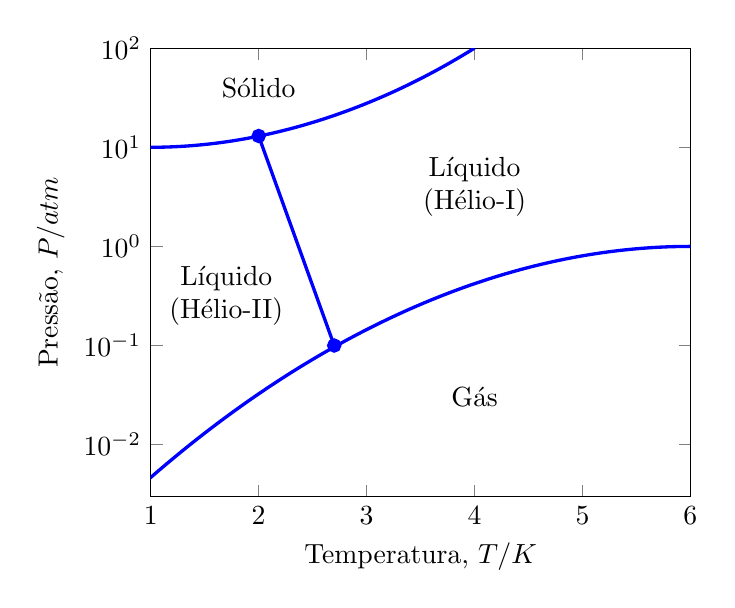
\begin{tikzpicture}
\begin{semilogyaxis}
    [
        grid = none,
        minor tick style={draw=none},
        ylabel = {Pressão, $P/\unit{atm}$},
        xlabel = {Temperatura, $T/\unit{K}$},
        ymin=0.003, ymax=100,
        xmin=1, xmax=6,
    ]       
    \draw [draw=blue, very thick]
        (axis cs: 6, 1) parabola 
        (axis cs: 0.8, 0.003);
    \draw [draw=blue, very thick]
        (axis cs: 1, 10) parabola 
        (axis cs: 4, 100);

    \addplot [ mark=*, color=blue, very thick ] coordinates
        { 
            (2.7, 0.1) 
            (2, 13) 
        };

    \node [anchor = center] at (axis cs: 2, 40) 
        { Sólido };
    \node [anchor = center] at (axis cs: 4, 0.03) 
        { Gás };
    \node [anchor = north, align = center] at (axis cs: 4, 10) 
        { Líquido \\ (Hélio-I) };
    \node [anchor = north, align = center] at (axis cs: 1.7, 0.8) 
        { Líquido \\ (Hélio-II) };
\end{semilogyaxis}
\end{tikzpicture}
